% !TeX root=main.tex
\pagenumbering{arabic}
\chapter{مقدمه}
\thispagestyle{empty}
	در سال‌های اخیر و با پیشرفت‌های چشمگیر در حوزه هوش مصنوعی، پردازش زبان طبیعی و پردازش تصویر مسئله‌هایی با کاربرد عملی در زندگی روزمره انسان‌ها طراحی شده است. یکی از مواردی که اخیرا مورد توجه قرار گرفته است، بحث پرسش و پاسخ تصویری می‌باشد. پرسش و پاسخ تصویری را می‌توان تعمیم یافته مسئله پرسش و پاسخ متنی دانست. در این مسئله یک تصویر و یک سوال در رابطه با تصویر به عنوان ورودی به سیستم داده می‌شود. سیستم با توجه به درک و تحلیلی که از متن و تصویر ورودی به دست‌ می‌آورد، یک پاسخ متنی به عنوان خروجی می‌دهد. 
	\newline
مسئله پرسش و پاسخ تصویری نسبت به پرسش و پاسخ متنی بسیار چالش برانگیزتر است. معمولا داده‌های تصویری نویز بیشتری نسبت به داده‌های متنی دارند. همچنین تحلیل و پردازش داده‌های تصویری با توجه به این که ابعاد بالاتری دارند، دشوار‌تر از داده‌های متنی می‌باشد. از طرفی تصویر اطلاعات بیشتری با خود به همراه دارد. گرچه تحلیل دقیق و صحیح تصویر در مقایسه با متن با چالش‌های بیشتری مواجه است اما تصویر اطلاعات و دانش بیشتری را با خود به همراه دارد. 
\section{کاربرد و اهمیت مسئله}
این مسئله کاربرد‌‌‌های زیادی در زندگی روزمره می‌تواند داشته باشد. از جمله کاربرد‌های مسئله برای کمک به افراد کم‌بینا یا نابینا در قالب اپلیکیشن‌های تلفن همراه می‌باشد \cite{gurari2018vizwiz}. افراد کم‌بینا یا نابینا به کمک این اپلیکیشن‌ها قادر خواهند بود درک بهتری از محیط پیرامون خود داشته باشند و تعامل بهتری با اطرافیان برقرار کنند. در شکل \ref{vqa-blind} نمونه‌ای از تصاویر به همراه سوالات کاربر و پاسخ سیستم هوشمند به سوالات قابل مشاهده است. در مواردی که تصویر اطلاعات مناسبی برای پاسخ‌گویی به سوال را  ندارد، پاسخ
\newline 
\lr{"unsuitable image"}
 از سیستم هوشمند دریافت می‌شود.

\begin{figure}[H]
	\center{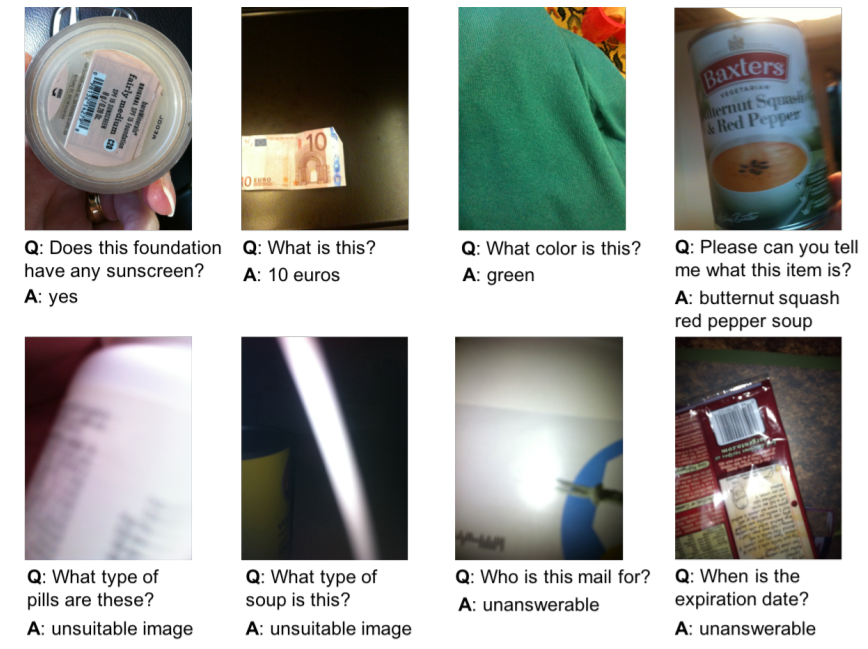
\includegraphics[width=0.9\linewidth]{images/vqa-blind.PNG}}
	\caption{نمونه‌ای از کاربرد پرسش و پاسخ تصویری برای افراد کم‌بینا و نابینا
		\cite{gurari2018vizwiz}}
	\label{vqa-blind}
\end{figure}

از موارد دیگر کاربرد‌های پرسش و پاسخ تصویری می‌توان از تفسیر تصاویر پیچیده پزشکی یاد کرد \cite{ImageCLEFVQA-Med2019}. این مسئله برای تشخیص بهتر و دقیق‌تر پزشکان از تصاویر رادیولوژی، می‌تواند مورد استفاده قرار بگیرد. همچنین در مواردی که پزشک در دسترس نباشد می‌توان از این ابزار برای تفسیر تصاویر استفاده کرد. نمونه از کاربرد پرسش و پاسخ تصویری در تحلیل تصاویر پزشکی در شکل\ref{vqa-med} قابل مشاهده است.
\begin{figure}[H]
	\center{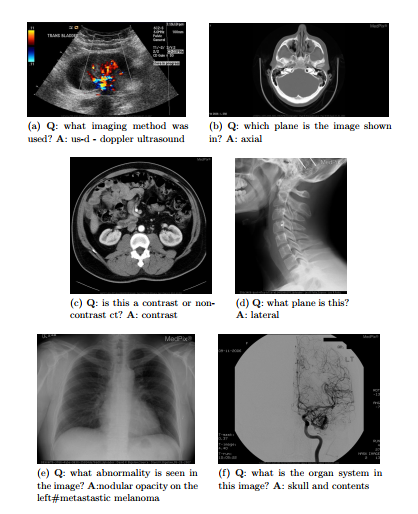
\includegraphics[width=0.8\linewidth]{images/vqa-med.PNG}}
	\caption{نمونه‌ای از کاربرد پرسش و پاسخ تصویری در پزشکی
		\cite{ImageCLEFVQA-Med2019}}
	\label{vqa-med}
\end{figure}

%\section{اهمیت و کاربرد مسئله}
\section{بررسی چالش های موجود در مسئله}
با توجه به اهمیت بحث پرسش و پاسخ تصویری در کمک به افراد کم‌بینا یا نابینا در زندگی روزمره و کمک به بهبود و تسهیل امور جاری روزانه، استفاده از مدل‌های آموزش دیده بر روی تلفن همراه یا وب‌سایت‌ها در قالب نرم‌افزار‌های کاربردی از اهمیت بالایی برخوردار است. از سوی دیگر اغلب تلفن‌های همراه قدرت پردازش و حافظه محدودی دارند. استفاده بهینه از منابع موجود بسیار حائز اهمیت است. بنابراین علاوه بر آموزش مدل مناسب که برای این مسئله به دقت قابل قبولی برسد، لازم است مدل ساخته شده از حجم مناسبی برخوردار بوده و قابل استفاده بر روی تلفن همراه با استفاده از کمترین منابع باشد. به طوری که کارکرد تلفن همراه را دچار اختلال نکند. 
\newline	 
با گسترش استفاده از شبکه‌های ترنسفورمر دقت‌های به دست‌آمده در مسئله پرسش و پاسخ تصویری به مقدار قابل قبولی رسیده است. اما شبکه‌های ترنسفورمری اغلب تعداد پارامتر‌های بالایی دارند. از این رو کوچک کردن مدل و فشرده سازی آن از جمله مسائل داغ مورد بررسی است.
در این پژوهش سعی شده است که هرس شبکه عصبی بر روی مسئله پرسش و پاسخ تصویری مورد بررسی قرار بگیرد و نتایج مدل فشرده شده با مدل اصلی مقایسه گردد. همچنین تاثیر فشرده سازی بر دقت مدل کاهش یافته و عملکرد آن بررسی ‌شود.

